\documentclass[10pt, letterpaper]{article} 

\usepackage{graphicx}
\usepackage{float}

\begin{document}
 
\textbf{Critical Thinking Questions}


\begin{figure}[H] % H need float and h doesn't
\centering
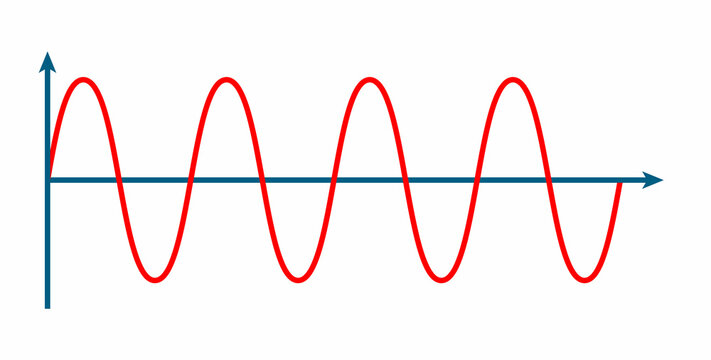
\includegraphics[width=0.4\textwidth]{limit}\\ % need graphicx
\caption{The Squeeze Theorem}
\end{figure}




\begin{enumerate}
\item Is it possible for a sequence to converge to two different numbers? If so, give an example. If not, explain why not.
\item Explain how to use partial sums to determine if a series converges or diverges. Give an example
\item Explain why $\int\limits_{1}^{\infty} f(x)\,dx$ and $\sum\limits_{n=1}^{\infty} a_n$ need not converge to the same value, even if they are both convergent.
\item  In your own words, explain the Alternating Series Remainder Theorem. How is this theorem useful?
\item Explain the difference between absolute and conditional convergence. Give an example of each.
\item The Ratio Test is inconclusive if $\displaystyle{\lim\limits_{n \to \infty} \left| \frac{a_{n+1}}{a_n} \right| =1}$. Give an example of one convergent series and one divergent series for which $\displaystyle{\lim\limits_{n \to \infty} \left| \frac{a_{n+1}}{a_n} \right| =1}$. Explain how you determined your examples.
\end{enumerate}


\end{document}




